\documentclass[spanish,12pt,letterpaper]{article}
\usepackage[margin=2cm]{geometry}
\usepackage[T1]{fontenc}
\usepackage{graphicx}
\usepackage{mathtools}
\usepackage{amssymb}
\usepackage{amsthm}
\usepackage{thmtools}
\usepackage{nameref}
\usepackage{babel}
\usepackage{mathrsfs}
\usepackage{hyperref}
\usepackage[linesnumbered,ruled,vlined]{algorithm2e}

\title{\textbf{Travelling Salesman Problem}}
\author{Victor Rosales Jaimes}
\date{}
\begin{document}
	\maketitle
	\section{Introducción}
	El Problema del Agente Viajero (TSP) es un desafío ampliamente reconocido en el campo de las ciencias de la computación, que implica la búsqueda de la ruta más corta que conecta un conjunto de ciudades y regresa al punto de partida. Este problema se clasifica como NP-duro, lo que significa que resulta computacionalmente intratable cuando se trata de un gran número de ciudades. Para abordar el TSP, se han desarrollado diversas heurísticas, que son algoritmos que proporcionan soluciones aproximadas, no necesariamente óptimas, pero que a menudo son adecuadas en la práctica. Una de estas heurísticas es el algoritmo de recocido simulado, que se inspira en el proceso de recocido utilizado en la metalurgia.\\
	
	
	El recocido simulado parte de una solución inicial y la mejora iterativamente mediante perturbaciones aleatorias. Estas perturbaciones son aceptadas si mejoran la solución o, en algunos casos, con cierta probabilidad si no lo hacen. A medida que avanza el algoritmo, la probabilidad de aceptar soluciones peores disminuye, lo que le permite escapar de óptimos locales y explorar de manera más exhaustiva el espacio de soluciones.\\
	
	La aceptación por umbrales es una variante eficiente del algoritmo de recocido simulado. En esta variante, la temperatura se utiliza como medida de la aleatoriedad en la realización de cambios en la solución, y se busca minimizar esta temperatura. A medida que la temperatura disminuye, la probabilidad de aceptar soluciones peores también se reduce, permitiendo al algoritmo escapar de óptimos locales y explorar más a fondo el espacio de soluciones. El criterio de aceptación en el recocido simulado puede basarse en un umbral, donde se acepta una perturbación si mejora la solución en una cantidad significativa, o en una distribución de probabilidad, donde la aceptación depende de la magnitud del cambio y un parámetro de temperatura que disminuye con el tiempo.
	\section{El problema}
	
	\subsection{La gráfica}
	
	Las ciudades en el mapa y sus conexiones estarán representadas por una gráfica ponderada $G(E, V), E \subset V \times V$; con una función de peso para las aristas $w: E \longrightarrow \mathbb{R}^{+}$ que representará la distancia entre cada par de ciudades. La gráfica que usaremos, aunque muy densa, no será completa.
	
	Sea $S \subset V ; S$ será la instancia de TSP que se querrá resolver. Para hacer más sencilla la optimización de este problema, se utilizará la gráfica completa $G_{S}\left(V_{S}, E_{S}\right)$, donde $V_{S}=S$ y $E_{S}=\{(u, v) \mid u, v \in S$ y $u \neq v\}$, con la función de peso aumentada $w_{S}: E_{S} \longrightarrow \mathbb{R}^{+}$ que se define como sigue:
	
	\subsubsection{Función de peso aumentada}
	
	Sea $w_{S}: E_{S} \longrightarrow \mathbb{R}^{+}$ tal que:
	
	\[
	w_{S}(u, v)=\left\{
	\begin{array}{cl}
		w(u, v) & \text { si }(u, v) \in E \\
		d(u, v) \times \text { máx }_{d}(S) & \text { en otro caso }
	\end{array}
	\right.
	\]
	
	donde $d(u, v)$ es la distancia natural entre dos vértices u y v; y máx ${ }_{d}(S)$ será la distancia máxima de $S$. Se puede consultar como calcular la distancia natural en \url{https://www.movable-type.co.uk/scripts/latlong.html} con la ligera diferencia en que usaremos metros en lugar de kilómetros.
	
	\subsubsection{Distancia máxima}
	
	La distancia máxima de $S$ se define como:
	
	\[
	\operatorname{max}_{d}(S)=\operatorname{max}\{w(u, v) \mid u, v \in S y(u, v) \in E\} \text {. }
	\]
	
	En otras palabras, $\operatorname{máx}_{d}(S)$ es la distancia máxima que existe entre pares de elementos de $S$ tales que estén conectados en $G$.

	
	\subsection{Soluciones}
	
	Dada una instancia $S$ de TSP, cualquier permutación de los elementos de $S$ es una solución al problema en $G_{S}$, porque $G_{S}$ es una gráfica completa.
	Aunque todas las permutaciones de $S$ son soluciones válidas en la gráfica $G_{S}$, esto no es cierto para $G$, que es donde realmente se desea resolver el problema. Una permutación será factible si y sólo si las aristas entre dos elementos consecutivos de la permutación existen en $E$ (siempre existen en $E_{S}$, porque $G_{S}$ es completa).
	
	Si al menos una arista entre dos elementos consecutivos de la permutación no existe en $E$, la solución será no factible.
	
	\subsection{Función de costo}
	
	La optimización de TSP necesitará una función de costo que se usará para evaluar qué tan buenas (o no) son las soluciones que el sistema encuentre. Como se quiere minimizar la distancia de la trayectoria que pase por todos los vértices, definimos $w_{S}$ de tal forma que las aristas que estén en $E_{S}$, pero no en $E$, tengan un peso mucho mayor que las aristas en $E$. Esto alentará al sistema a tratar de descartar aristas que no estén en $G$ para entonces encontrar soluciones factibles.
	
	Para poder comparar, aunque sea burdamente, las evaluaciones a soluciones factibles de instancias de TSP diferentes, vamos a normalizar la función de costo. Para esto necesitaremos un normalizador.
	
	\subsubsection{Normalizador}
	El normalizador de $S$ (denotado por $\mathscr{N}(S)$ ) está definido como:
	
	\[
	\mathscr{N}(S)=\sum_{d \in L^{\prime}} d .
	\]
	
	En otras palabras, y suponiendo que $|S|=k$, el normalizador de $S$ es la suma de las $k-1$ aristas más pesadas en $E$ formadas de elementos de $S$.
	
	\subsubsection{Función de costo}
	
	Sea $S \subset V$ una instancia de TSP; la función de costo $f$ de una permutación $P=v_{\rho(1)}, \ldots, v_{\rho(k)}$ de los elementos de $S$ se define como:
	
	\[
	f(P)=\frac{\sum_{i=2}^{k} w_{S}\left(v_{\rho(i-1)}, v_{\rho(i)}\right)}{\mathscr{N}(S)} .
	\]
	
	Ésta es la función que se buscará optimizar. Además considerando esta función diremos que una solución es factible si el valor de la función de costo esta entre $0$ y $1$.
	\subsection{Solución vecina}
	 Sea $S$ una instancia de TSP y $P=v_{\rho(1)}, \ldots, v_{\rho(k)}$ y $P^{\prime}=v_{\sigma(1)}, \ldots, v_{\sigma(k)}$ dos permutaciones de los elementos de $S$.
	
	Diremos que $P$ y $P^{\prime}$ son vecinas si y sólo si existen dos índices $1 \leq s, t \leq k, s \neq t$, tales que:
	
	- $v_{\rho(i)}=v_{\sigma(i)}$ si $i \notin\{s, t\}, y$
	
	- $v_{\rho(s)}=v_{\sigma(t)} y v_{\rho(t)}=v_{\sigma(s)}$.
	
	En otras palabras, dos soluciones serán vecinas si intercambiando dos elementos de la primera se obtiene la segunda.
	
	\section{Aceptación por umbrales}
	La heurística de Recocido Simulado (Simulated Annealing) fue propuesta por Scott Kirkpatrick, Daniel Gelatt y Mario Vecchi en 1983. La idea de la heurística es emular la técnica metalúrgica de recocido que se utiliza para reducir los defectos en metales.
	
	Gunter Dueck y Tobias Scheuer crearon en 1990 la variante del Recocido Simulado que denominaron Aceptación por Umbrales (Threshold Accepting), que en general se considera más sencilla de implementar.
	
	\subsection{La heurística}
	Dado un problema de optimización $\mathscr{P}$ clasificado como NP-duro, consideramos el conjunto de posibles soluciones $S$ y una función objetivo $f: S \rightarrow \mathbb{R}^{+}$, donde $0 \leq f(s) < \infty$ para cualquier solución $s \in S$.
	
	El proceso comienza con la elección de una temperatura inicial $T \in \mathbb{R}^{+}$ y una solución inicial $s$ obtenida de manera aleatoria. Luego, de forma aleatoria, se busca una solución vecina $s^{\prime}$ tal que $f\left(s^{\prime}\right) \leq f(s) + T$. Si se encuentra una solución $s^{\prime}$ que cumple esta condición, se actualiza $s$ para que sea igual a $s^{\prime}$, y esta nueva solución $s^{\prime}$ se considera aceptada.
	
	Este proceso se repite mientras la temperatura $T$ disminuye gradualmente, siguiendo una serie de condiciones predefinidas. La heurística puede terminar cuando se cumple una de las siguientes condiciones:
	
	\begin{enumerate}
		\item La temperatura $T$ cae por debajo de un valor umbral $\varepsilon$ (para $\varepsilon > 0$ muy pequeña).
		\item Se ha generado un número determinado de soluciones aceptadas.
		\item Se satisfacen otras condiciones predefinidas específicas del problema.
	\end{enumerate}
	
	La heurística de aceptación por umbrales busca encontrar soluciones óptimas o de alta calidad mediante un proceso de exploración y explotación que depende de la temperatura y de las soluciones vecinas encontradas. Este enfoque puede ser útil para abordar problemas NP-duros donde la búsqueda exhaustiva no es viable.

	\subsection{Algoritmos}
	Las condiciones para decrementar la temperatura $T$ estarán dadas por el
	comportamiento de lo que se llamarán lotes; un lote será un número determinado de soluciones aceptadas. En este algoritmo usamos $L\in \mathbb{N}$ que se obtiene por vías experimentales, en cuanto a nuestras experimentaciones consideramos que lotes de tamaño $2000$ son adecuados.\\
	
	\begin{algorithm}[H]
		\caption{CALCULALOTE(T, s)}
		\KwData{Temperatura $T$, solución $s$}
		$c \leftarrow 0$\;
		$r \leftarrow 0.0$\;
		\While{$c < L$}{
			$s' \leftarrow$ VECINO($s$)\;
			\If{$f(s') \leq f(s) + T$}{
				$s \leftarrow s'$\;
				$c \leftarrow c + 1$\;
				$r \leftarrow r + f(s')$\;
			}
		}
		\KwResult{Promedio de las soluciones aceptadas $r/L$ y última solución aceptada $s$}
	\end{algorithm}
	\hfill \break		
	
	Sabiendo calcular lotes, se puede definir el algoritmo principal de la aceptación por umbrales. Este algoritmo hace uso de ciertas constantes que listamos a continuación:
	\begin{itemize}
		\item $\epsilon$ : es un cero virtual que al que se desea llegar al decrementar la temperatura.
		\item  $\phi$: es la tasa de enfriamiento del sistema, es decir, es el factor por el cual se multiplicará la temperatura $T$ para ir disminuyendola.
	\end{itemize}
	
	\begin{algorithm}
		\caption{ACEPTACIONPORUMBRALES(T, s)}
		\KwData{Temperatura inicial $T$ y solución inicial $s$}
		$p \leftarrow 0$\;
		\While{$T > \varepsilon$}{
			$q \leftarrow \infty$\;
			\While{$p \leq q$}{
				$q \leftarrow p$\;
				$p, s \leftarrow$ CALCULALOTE($T$, $s$)\;
			}
			$T \leftarrow \phi T$ \;
		}
		\KwResult{Solución final $s$}
	\end{algorithm}
	
	\subsection{Temperatura inicial}
	La temperatura inicial afecta en gran medida el comportamiento del sistema; se quiere una temperatura inicial suficientemente 	alta para evitar caer en un mínimo local muy temprano; pero suficientemente baja para que el sistema no tarde demasiado en terminar. Existe un algoritmo para determinar este aunque contradictoriamente recibe un temperatura:\\
	
	\begin{algorithm}
		\caption{TEMPERATURAINICIAL($s$, $T$, $P$)}
		\KwData{Solución inicial $s$, temperatura inicial $T$, porcentaje objetivo $P$}
		$p \leftarrow$ PORCENTAJEACEPTADOS($s$, $T$)\;
		\If{$|P - p| \leq \varepsilon_P$}{
			\KwResult{$T$}
		}
		\If{$p < P$}{
			\While{$p < P$}{
				$T \leftarrow 2T$\;
				$p \leftarrow$ PORCENTAJEACEPTADOS($s$, $T$)\;
			}
			$T_1 \leftarrow T/2$\;
			$T_2 \leftarrow T$\;
		}
		\Else{
			\While{$p > P$}{
				$T \leftarrow T/2$\;
				$p \leftarrow$ PORCENTAJEACEPTADOS($s$, $T$)\;
			}
			$T_1 \leftarrow T$\;
			$T_2 \leftarrow 2T$\;
		}
		\KwResult{BUSQUEDABINARIA($s$, $T_1$, $T_2$, $P$)}
	\end{algorithm}
	
	\begin{algorithm}
		\caption{PORCENTAJEACEPTADOS($s$, $T$)}
		\KwData{Solución $s$, temperatura $T$}
		$c \leftarrow 0$\;
		\For{$i \leftarrow 1$ \KwTo $N$}{
			$s' \leftarrow$ VECINO($s$)\;
			\If{$f(s') \leq f(s) + T$}{
				$c \leftarrow c + 1$\;
				$s \leftarrow s'$\;
			}
		}
		\KwResult{Porcentaje de soluciones aceptadas $\frac{c}{N}$}
	\end{algorithm}
	
	\begin{algorithm}
		\caption{BUSQUEDABINARIA($s$, $T_1$, $T_2$, $P$)}
		\KwData{Solución $s$, temperaturas iniciales $T_1$ y $T_2$, porcentaje objetivo $P$}
		$T_m \leftarrow (T_1 + T_2)/2$\;
		\If{$T_2 - T_1 < \varepsilon_P$}{
			\KwResult{$T_m$}
		}
		$p \leftarrow$ PORCENTAJEACEPTADOS($s$, $T_m$)\;
		\If{$|P - p| < \varepsilon_P$}{
			\KwResult{$T_m$}
		}
		\If{$p > P$}{
			\KwResult{BUSQUEDABINARIA($s$, $T_1$, $T_m$, $P$)}
		}
		\Else{
			\KwResult{BUSQUEDABINARIA($s$, $T_m$, $T_2$, $P$)}
		}
	\end{algorithm}
	
	\newpage
	\section{Sistema}
	\subsection{Instancia}
	En el contexto de este estudio, hacemos referencia a una instancia personalizada del Problema del Agente Viajero (TSP) que se encuentra almacenada en una base de datos. Esta instancia contiene información detallada sobre las ciudades que la componen, como sus nombres, países de ubicación, población y coordenadas geográficas (latitud y longitud). Además, la base de datos contiene datos relacionados con los costos o distancias entre algunos pares de ciudades, aunque no necesariamente todas las ciudades están conectadas directamente entre sí. Esta base de datos se utiliza de manera global, y a partir de ella, se obtienen subconjuntos de ciudades y conexiones para crear instancias específicas.
	\\
	
	En el marco de la experimentación, consideramos dos instancias distintas: una con 40 ciudades y otra con 150 ciudades.
	
	
	\subsection{Constantes del sistema}
	El sistema se ha implementado en Java, y en él se han implementado los dos algoritmos descritos en las secciones 3.2 y 3.3. A continuación, se enumeran las variables utilizadas en el sistema, que se han determinado de manera experimental y se ha notado que son las más adecuadas para este caso particular:
	
	\begin{itemize}
		\item Tamaño de lote ($L$): $2000$
		\item Tasa de enfriamiento ($\phi$): $0.9$
		\item Épsilon ($\varepsilon$): $0.00001$
		\item Temperatura inicial: $1000$
		\item Porcentaje objetivo: $0.85$
		\item Épsilon $P$: $0.1$
	\end{itemize}
	
	Todos los valores mencionados anteriormente se definen como constantes.
	\subsection{Entrada}
	El sistema incorpora un componente aleatorio al buscar una solución vecina. Por esta razón, el sistema recibe como entrada un número entero que funciona como semilla para el generador de números aleatorios, lo que permite que los resultados sean reproducibles.
	
	Además, se requiere una lista de números (identificadores en la base de datos), la cual se proporciona mediante el nombre del archivo que la contiene.
	
	En resumen, el sistema recibe los siguientes datos de entrada:
	\begin{itemize}
		\item Nombre del archivo que contiene una lista de números separados por comas.
		\item Una semilla aleatoria.
	\end{itemize}
	
	
	\section{Resultados}
	Como mencionamos en la sección anterior, tenemos dos instancias: una con 40 ciudades y otra con 150 ciudades.
	
	Utilizando las constantes del sistema definidas en la sección 4.2, realizamos pruebas con $10,000$ semillas en la instancia de 40 ciudades. Cada semilla produjo resultados distintos, y determinamos que el costo mínimo obtenido por el sistema se alcanza cuando el valor de la semilla es $5123$, con un valor de la función de costo de $0.250989$.
	
	En el caso de la instancia de 150 ciudades, probamos $1,000$ semillas y determinamos que el costo mínimo se alcanza cuando el valor de la semilla es $82$, con un costo de $0.151461$.
	
	A continuación, se presenta un gráfico que representa la relación entre el costo de la solución y la iteración, conforme la temperatura disminuye:
	
	
	\begin{figure}[ht]
		\begin{minipage}[b]{0.5\linewidth}
			\centering
			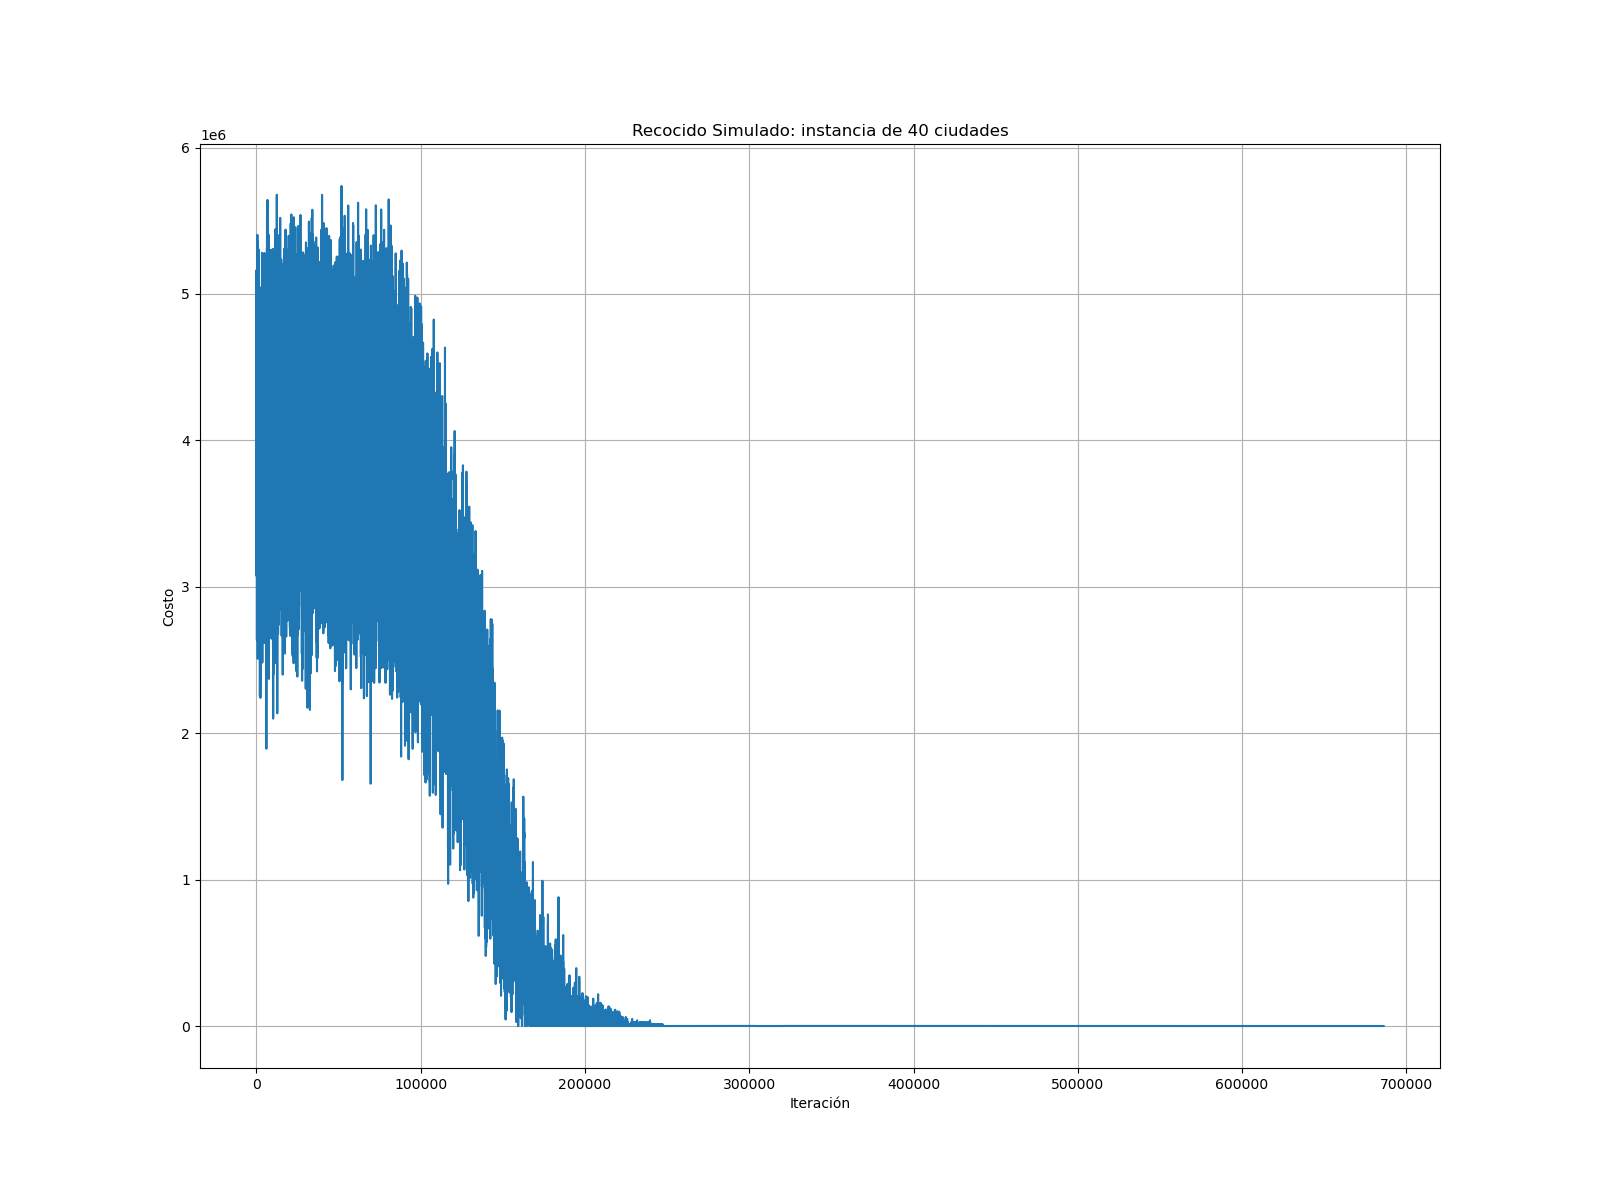
\includegraphics[width=1\linewidth]{images/40.png}
			\caption{Instancia de 40 ciudades}
			\label{fig:40ciudades}
		\end{minipage}
		\begin{minipage}[b]{0.5\linewidth}
			\centering
			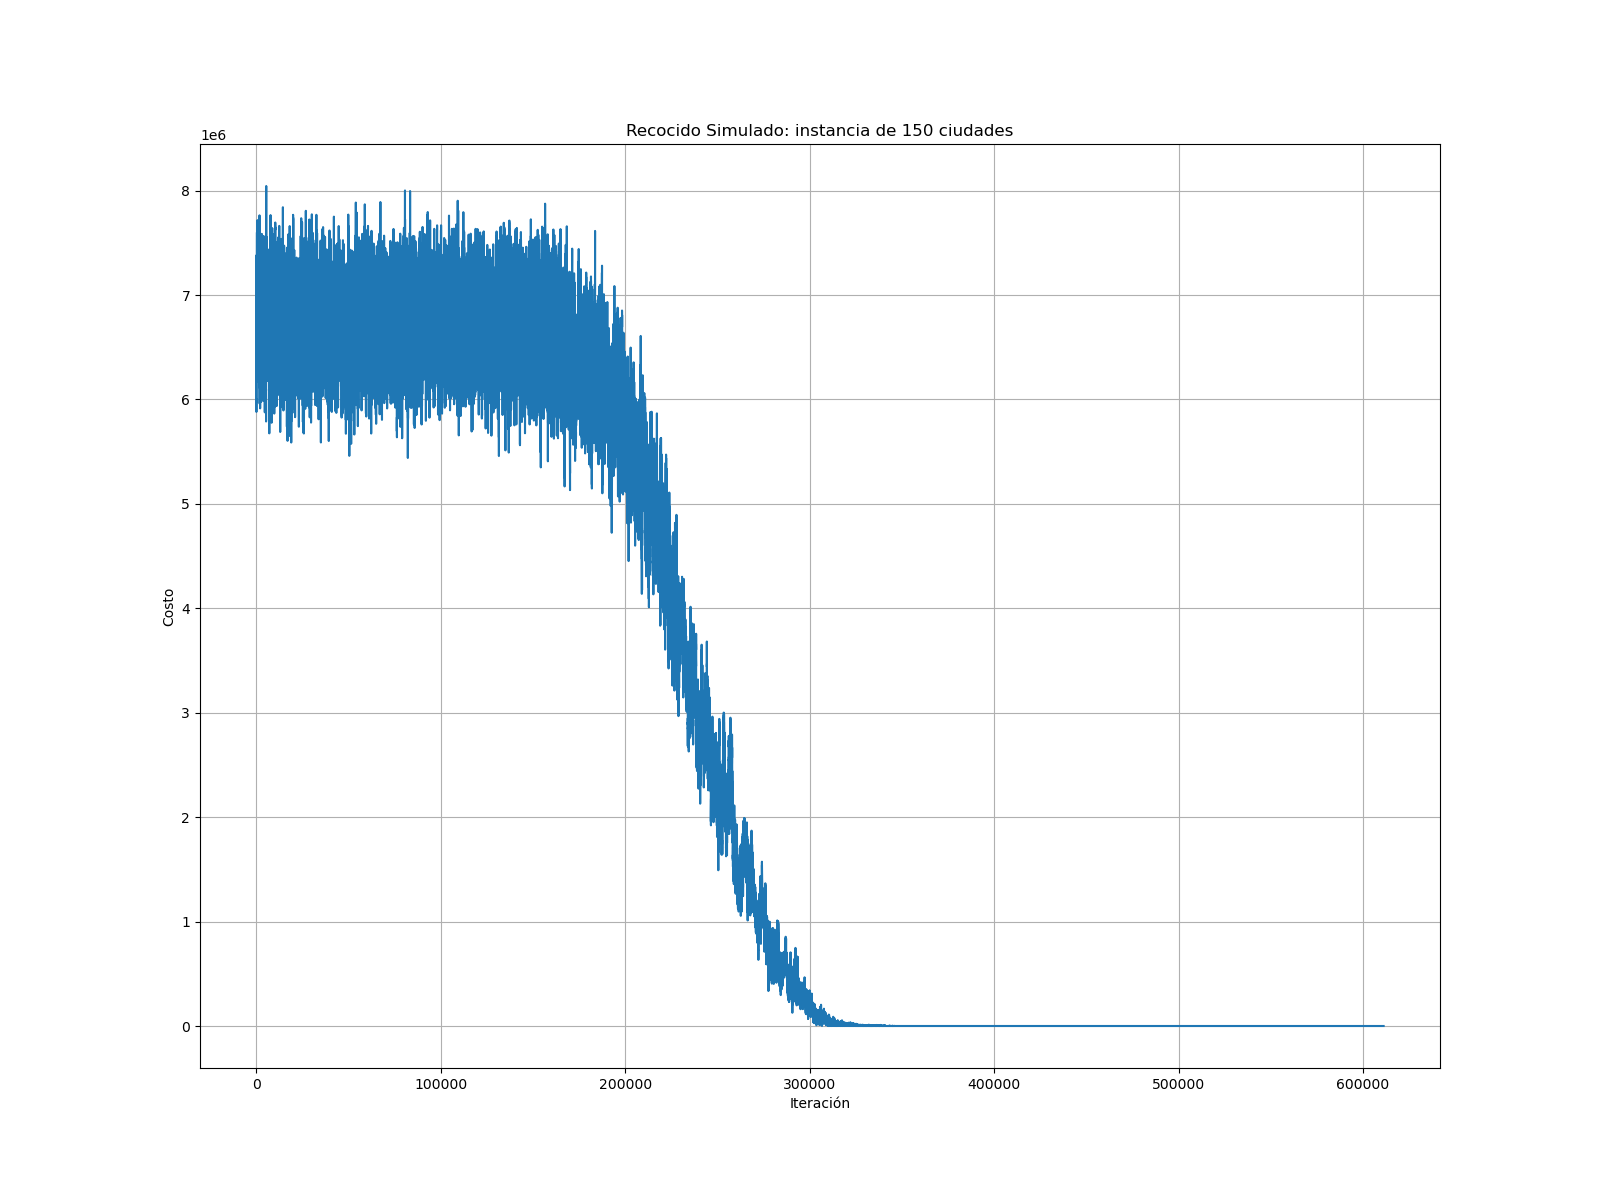
\includegraphics[width=1\linewidth]{images/150.png}
			\caption{Instancia de 150 ciudades}
			\label{fig:150ciudades}
		\end{minipage}
	\end{figure}

	
\end{document} 